%!TEX root = ../thesis.tex

\section{Principles and Methods}
% Motion Illustration
% \bjoern{this section is too long for the work it does - more than page! Shorten.}
% \dan{I did some trimming, now a few lines more than a column without comments (not counting figure).}
% \dan{The main takeways after reading this section should be: 1) the style of illustration our system supports matches what people actually need; 2) current practices are slow and/or require specialized skills; 3) automating the first part of the process is most important: generating (and experimenting with) keyframe illustrations with motion annotations from real time demonstrations. } \bjoern{Yes!}

To understand motion illustration design and production, we surveyed related literature, studied found examples, and interviewed individuals who create such illustrations.

\subsection{Design Principles}
%to evaluate five general methods
Cutting~\cite{cutting_representing_2002} argues that superimposing vector-like lines on an image satisfies four important criteria: it evokes a feeling of motion, the object undergoing motion is clearly represented, the direction of motion is clear, and the magnitude of motion is conveyed with reasonable precision. To complement this metaphoric representation, Cutting also argues for the more literal method of multiple stroboscopic images, which satisfies all criteria except clear motion direction. McCloud~\cite{mccloud_understanding_1994} provides further arguments and examples for using these methods in the field of comic illustration, and notes communication benefits when they are combined.

To examine how professional illustrators use motion lines and stroboscopic images, we gathered examples from sources like user manuals, gesture-based games, safety guides, % (e.g., for airplane safety or weight training),
illustration compendia (e.g.,~\cite{mijksenaar1999open}) and how-to books (e.g.,~\cite{greenberg2012sketching}).
%
We found Cutting's notion of vector-like lines are almost always rendered with an arrowhead % with of a clear head at the end of a line tracing the motion path.
in a variety of styles (heads, weights, colors) with strokes typically two-dimensional, smooth, and offset to avoid occluding the object.
Stroboscopic images can be overlapping or spatially distributed, and change in transparency or shading to convey time.
The most common style for depicting the object undergoing motion is a simplified black-and-white contour drawing, but filled silhouettes and flat-shaded colour can also be found -- using full color photographic detail is rare.
%
By carefully removing extraneous details, such techniques help readers focus on only the salient, abstract information.
% \bjoern{Add WHY - omit extraneous details to focus on salient features.}

% These methods can be used with the object undergoing motion rendered as a full color photo or as a stylized illustration with reduced detail. \dan{One or two sentence giving benefits of using illustrations over photos that adds more detail to the general argument in the introduction [references in Pat Hanrahan's lecture slides, maybe Buxton's sketching book ] } Early in the 90s, Dooley and Cohen designed a method to generate line illustrations from geometric model \cite{Dooley:1990:AIG:91394.91422, Dooley:1990:AIG:91385.91422}. This...

% http://vis.berkeley.edu/courses/cs294-10-fa13/wiki/index.php/Conveying_Shape:_Lines#readings

% NOTES

% - -

% Cutting (2002)
% (this article is amazing)

% 4 criteria for
% evocativeness: a feeling of movement
% clarity: can the object undergoing motion be easily identified
% direction: where is the object moving?
% precision: what is the magnitude of the motion?

% 5 general techniques to convey motion:
% dynamic balance: choose a pose to convey sense of movement (questionable direction, poor precision)
% affine shear: leaning into the direction of movement (evocative and somewhat clear, Cutting says direction is good(?))
%  motion blur (only evocative)
% stroboscopic images: “Motion as time discretely sampled” (poor direction (?) )
% arrows (action lines, speed lines), a more literal representation of the motion vector … Cutting says this is best: (evocative, clear, direction, precise)

% literal representations of motion (strobing, motion blur) and metaphorical (arrows, action lines)

% - -

% McCloud (1993)
% (need to read more)

% talks about benefits of combining stroboscopic and action-line (headless arrows)

% - -

% OpenHere

% Interesting history of the arrow (p19) -- it's a somewhat recent convention.

% kind of off-the-cuff description of different arrow and lines types on p102 (e.g. dotted lines indicate stages of movement)

% many techniques for visual instructions come form cartoons (e.g. lines for movement)

% - -

% Pat Hanrahan’s lecture slides (provides references to justify using illustration over photos ssaying  ``Illustrations often better than photographs, they enhance important features and emphasize unimportant detail''

% - -

% Buxton, Sketching Interaction

% (didn’t find anything relevant beyond comments about arrows being good for conveying motion … our work isn't really about sketching, we're illustrating.)


\subsection{Interviews: Methods Used In the HCI Community}
% https://docs.google.com/document/d/1TisNlsFUYQ3a-BuqryRv8qmyp3La-qLj-j3hN4PyVS8/edit
% \bjoern{The challenge here is that HCI researchers with Illustrator chops are MUCH closer to experienced designers than the general population. So using HCI authors to make an argument about ``non-designers'' is problematic. I took it out.}
% The examples we gathered above are produced by professional illustrators, but many other people create motion illustrations as part of their work --
% A central goal of our system is to empower individuals to rapidly create professional-quality motion illustrations.
To understand current creation methods, we conducted video interviews with six Human-Computer Interaction researchers with experience creating motion illustrations.
%
Conveying movement for interaction is common in HCI publications. We found 100 motion illustrations in 58 recent papers.

%We conducted interviews with 6 researchers with experience creating motion illustrations.
% We surveyed papers published between years 2005 to 2014 that contained motion illustrations in venues such as CHI, UIST, and MobileHCI -- we found whole-body motions, such as play in an interactive room and large display interactions; and  hand motions, such as smartphone interactions. We conducted video interviews with six authors of such papers about their process.

% and found
%100 motion illustration figures in 58 papers. From a pool of authors who created illustrations in two or more of these papers, we invited 6 to share their experiences (aged 25-43, all males: 3 professors, 2 industry researchers, 1 graduate student).
%Two participants had some design or art background.
%
%Interviews were conducted by video conference for one hour. The discussion focused on the creation process for 2 to 4 figures which we selected from the interviewee's papers. Selected figures for two interviewees were whole-body motions, such as game play in a room space and large display interaction; figures for the rest were hand motions, such as smartphone or hand-held device interaction.

\subsubTitleBold{Findings}
% in 3 categories: tools and creation process, motivations, and struggles
% Several authors emphasized the importance of concision and focus: they introduced important concepts via illustrations with unnecessary details excluded, like faces, clothing, and backgrounds. Establishing a consistent visual style was important to reuse graphic elements. %, especially for operating mobile devices.
%
All interviewees used a similar methodology to create motion illustrations: they took still photographs of people performing actions, traced outlines using Adobe Photoshop (4/6) or Illustrator (2/6), then added graphic annotations to convey motion. %One interviewee with design expertise sometimes drew illustrations from scratch.
%All interviewees mentioned the importance of iterating illustrations. Often preliminary versions were created for an early draft and refined later.
% 4 of the 6 interviewees used Photoshop, while 2 used Illustrator; 3 solely used a mouse while 3 used a stylus as a main input device.
%
All mentioned that it was time-consuming to set up scenes and poses, take and trace photos, then add details like arrow placement while maintaining a consistent style. Typical creation times were estimated between 10 minutes to a few hours.
They also noted how difficult it was to make adjustments: changing the pose or viewpoint essentially meant starting over again with new source photos and re-tracing.
Yet, identifying the best pose and viewpoint ahead of time is difficult and it often took several iterations to yield an illustration suitable for publication.
% \dan{I added the last sentence, Peggy please confirm that aligns with what you heard in the interviews ... I know at least I said that ;)}

\begin{figure}[t]
  \centering
  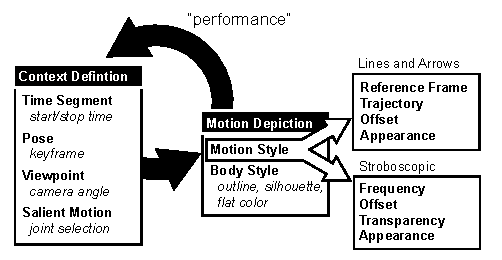
\includegraphics[width=\columnwidth]{\demodraw/fig/designdimensions}
  \caption{Canonical authoring workflow consisting of a Context Definition task then a Motion Depiction task. Design decisions associated with a task shown in bold with design parameters in italics.}
  \label{fig:designspace}
\end{figure}

\subsection{Design Space Goals and Workflow}

Based on the above, we derive a canonical workflow to motivate the central design goal for our system.
Authors face two primary illustration tasks (Figure~\ref{fig:designspace}):
\textit{defining the context} for portraying motion like the view of the body and salient aspects of motion;
and \textit{exploring a style of motion depiction} by choosing styles like lines-and-arrows or stroboscopic, then adjusting related style parameters.
These tasks and the underlying design parameters are highly interdependent, so authoring motion illustrations is necessarily an iterative process.
This means that changes to one task parameter often leads to re-evaluating and changing the other.
The problem with current methods, is that context is mostly ``performed'' using a time-consuming process of taking photos and manually tracing them.
%
Therefore, the central design goal of our system is to make context definition  low effort and iterative by using interactive demonstrations for automated context definition.

% enable low-effort iteration within, and between, the three identified tasks.

% %When creating illustrations, there are two primary tasks: 1) \textit{selecting the body context} and 2) body and motion \textit{depiction} (Figure~\ref{fig:designspace}).
% %\dan{I think ``context'' and ``depiction'' capture what people do, but maybe there are better terms.} \bjoern{yeah i don't understand them.}
% Performance capture involves recording suitable primary material to analyze and visualize. Identifying salient aspects
% %Selecting the body context
% involves segmenting a motion into steps, selecting key poses,
% %adjusting the camera angle to optimize the depiction of the pose and motion annotations,
% and identifying joints as salient motion for annotation. Depiction involves selecting a body visualization style, picking a motion visualization style (lines-and-arrows or stroboscopic), and adjusting many specific motion style parameters.
% These design parameters are all highly interdependent.
% %which is why the sequential and manual creation processes used by our interviewees is so time-consuming.


%Since current methods for the context setting task are time-consuming and inflexible, our system places extra focus on enabling rapid iteration.

Designing a system to capture interactive demonstrations of \textit{any} body movement also poses an input challenge.
Since  body movements form the demonstration itself, also issuing application commands with a body gesture introduces ambiguity.
Using a hand held device, touch screen, or any conventional input is not ideal since performing requires open space and full freedom of movement.
For these reasons, we use a multi-modal voice and gesture interaction style traced back to Bolt's Put-That-There~\cite{Bolt:1980:PutThatThere}. Like Bolt, we use voice for commands like \iquote{start} and \iquote{stop} with body movements providing command parameters in the form of the recorded demonstration, and for setting parameter context with utterances like \iquote{one, two, three, four} to label step-by-step segments.

%\peggy{We did not mention the reason we chose speech/voice for input. I briefly mentioned it in Pipeline in one sentence, but do we want to add a subsection here or mention in Introduction?}
%\dan{I added the paragraph above.}

% In addition, using manual techniques like photography or general purpose drawing tools like Adobe Illustrator means task parameters are highly under-constrained. This means the burden of upholding good design is placed on the non-expert user.
% A second goal of our system is to constrain the parameter space so that visualization principles are maintained.
% \dan{not sure if we do this second goal well}


% Lines: We may want to mention smoothing here? Several participants thought our system nicely smoothed the curves/arc (but should also straighten lines) even if their demo or Kinect mocap was not perfect.
% - Arrows: Double-headed arrows indicate repetition. DemoDraw does not adjust this automatically, but authors can manually change it to assign the intention.
% - Stroboscopic: also transparency? (had some meaning beyond appearance)
% - Sequencing: 1) DemoDraw generates the step-by-step diagrams based on motion segments, but also 2) Stroboscopic effect indicates the sequence of 2+ poses.

% \bjoern{Somewhere in the prior section or following section: Describe the design space of decisions one has to make to design an effective illustration. And argue that this is necessarily an iterative process where changes to one dimension may lead the designer to re-evaluate and change other dimensions. This is not possible with the current manual workflow starting with photos - authors are locked into a linear pipeline.}

% provide parameters, flexibility, direct manipulation, iterative design process


